\chapter{EXPERIMENTAL SETUP}

\section{Hardware setup}

The set-up comprises an Arduino microcontroller along with GSM module SIM 300A and a GPS shield. The Arduino is supplied with a 5V power supply. The GSM module must be given an external power supply and it should also be connected to the Arduino. The TX and RX pins of the Arduino are connected to the corresponding pins in the GSM module. The GPS shield also requires similar connections as the GSM module. As there are only one TX and RX pins on the Arduino, we must change other pins to act as another TX and RX pair. The GSM module also requires a functioning SIM card to be put in the slot given in the module. 

\section{Software setup}

The set-up consists of an application server which listens for any accident reported to it. Once an accident is reported, it generates alerts to be sent to the emergency contact of the user and the server also make use of a push notification microservice to notify users of the app about the accident.


\pagebreak
\section{Setup}

\begin{figure}[h!]
	\centering
	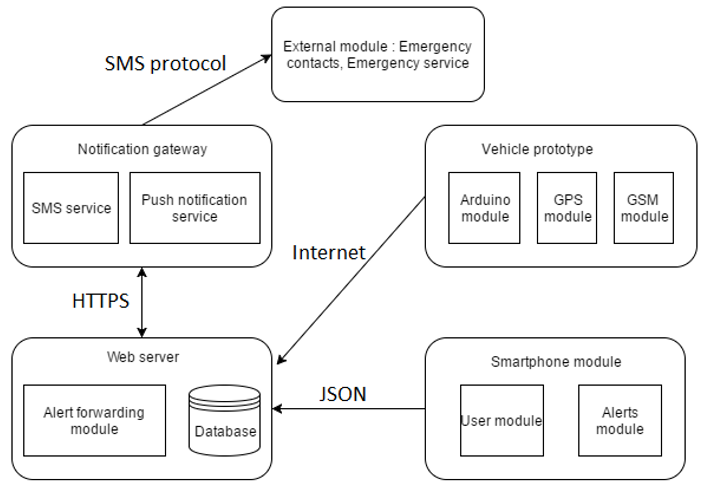
\includegraphics[scale=0.7]{arch}
	\caption{Setup}
	\label{fig:arch}
\end{figure}
